\documentclass[]{article}
\usepackage{lmodern}
\usepackage{amssymb,amsmath}
\usepackage{ifxetex,ifluatex}
\usepackage{fixltx2e} % provides \textsubscript
\ifnum 0\ifxetex 1\fi\ifluatex 1\fi=0 % if pdftex
  \usepackage[T1]{fontenc}
  \usepackage[utf8]{inputenc}
\else % if luatex or xelatex
  \ifxetex
    \usepackage{mathspec}
  \else
    \usepackage{fontspec}
  \fi
  \defaultfontfeatures{Ligatures=TeX,Scale=MatchLowercase}
\fi
% use upquote if available, for straight quotes in verbatim environments
\IfFileExists{upquote.sty}{\usepackage{upquote}}{}
% use microtype if available
\IfFileExists{microtype.sty}{%
\usepackage{microtype}
\UseMicrotypeSet[protrusion]{basicmath} % disable protrusion for tt fonts
}{}
\usepackage[margin=1in]{geometry}
\usepackage{hyperref}
\hypersetup{unicode=true,
            pdftitle={Predicting treatment response using shallow whole genome sequencing of cell-free DNA using in patients with metastatic Her2+ve breast cancer.},
            pdfauthor={Alistair Martin and Emma Beddowes and Mario Ortega Duran and others and Carlos Caldas},
            pdfborder={0 0 0},
            breaklinks=true}
\urlstyle{same}  % don't use monospace font for urls
\usepackage{longtable,booktabs}
\usepackage{graphicx,grffile}
\makeatletter
\def\maxwidth{\ifdim\Gin@nat@width>\linewidth\linewidth\else\Gin@nat@width\fi}
\def\maxheight{\ifdim\Gin@nat@height>\textheight\textheight\else\Gin@nat@height\fi}
\makeatother
% Scale images if necessary, so that they will not overflow the page
% margins by default, and it is still possible to overwrite the defaults
% using explicit options in \includegraphics[width, height, ...]{}
\setkeys{Gin}{width=\maxwidth,height=\maxheight,keepaspectratio}
\IfFileExists{parskip.sty}{%
\usepackage{parskip}
}{% else
\setlength{\parindent}{0pt}
\setlength{\parskip}{6pt plus 2pt minus 1pt}
}
\setlength{\emergencystretch}{3em}  % prevent overfull lines
\providecommand{\tightlist}{%
  \setlength{\itemsep}{0pt}\setlength{\parskip}{0pt}}
\setcounter{secnumdepth}{0}
% Redefines (sub)paragraphs to behave more like sections
\ifx\paragraph\undefined\else
\let\oldparagraph\paragraph
\renewcommand{\paragraph}[1]{\oldparagraph{#1}\mbox{}}
\fi
\ifx\subparagraph\undefined\else
\let\oldsubparagraph\subparagraph
\renewcommand{\subparagraph}[1]{\oldsubparagraph{#1}\mbox{}}
\fi

%%% Use protect on footnotes to avoid problems with footnotes in titles
\let\rmarkdownfootnote\footnote%
\def\footnote{\protect\rmarkdownfootnote}

%%% Change title format to be more compact
\usepackage{titling}

% Create subtitle command for use in maketitle
\providecommand{\subtitle}[1]{
  \posttitle{
    \begin{center}\large#1\end{center}
    }
}

\setlength{\droptitle}{-2em}

  \title{Predicting treatment response using shallow whole genome sequencing of cell-free DNA using in patients with metastatic Her2+ve breast cancer.}
    \pretitle{\vspace{\droptitle}\centering\huge}
  \posttitle{\par}
    \author{Alistair Martin and Emma Beddowes and Mario Ortega Duran and others and Carlos Caldas}
    \preauthor{\centering\large\emph}
  \postauthor{\par}
      \predate{\centering\large\emph}
  \postdate{\par}
    \date{28 May, 2019}


\begin{document}
\maketitle

\begin{verbatim}
## 'select()' returned 1:many mapping between keys and columns
\end{verbatim}

\hypertarget{abstract}{%
\section{Abstract}\label{abstract}}

\hypertarget{introduction}{%
\section{Introduction}\label{introduction}}

\hypertarget{methods}{%
\section{Methods}\label{methods}}

\hypertarget{results}{%
\section{Results}\label{results}}

\hypertarget{discussion}{%
\section{Discussion}\label{discussion}}

\hypertarget{conclusion}{%
\section{Conclusion}\label{conclusion}}

\clearpage

\hypertarget{tables}{%
\section{Tables}\label{tables}}

\begin{tabular}{l|l|r}
\hline
Measure & value & N\\
\hline
Age at primary diagnosis & (0,40] & 4\\
\hline
 & (40,50] & 10\\
\hline
 & (50,60] & 17\\
\hline
 & (60,70] & 9\\
\hline
 & (70,120] & 8\\
\hline
Race & White & 47\\
\hline
 & Unknown & 1\\
\hline
Primary receptor status & ER Negative, HER2 Positive & 8\\
\hline
 & ER Positive, HER2 Positive & 36\\
\hline
 & Indeterminate & 3\\
\hline
Grade at primary diagnosis & I & 1\\
\hline
 & II & 17\\
\hline
 & III & 27\\
\hline
 & Unknown & 3\\
\hline
Vital status & Alive & 13\\
\hline
 & Deceased & 35\\
\hline
\end{tabular}

Measure Comparison

Time Dependent Cox Model

Progression Free Survival

ichorCNA.default

0.860***

1.370***

(0.210)

(0.437)

t.Mad

0.503***

-0.645

(0.161)

(1.240)

ichorCNA.low

0.383***

0.366

(0.126)

(0.517)

z.OR

0.444***

-0.358

(0.162)

(0.730)

absolute

0.432***

0.122

(0.165)

(0.258)

AIC

135.1

143.9

145

145.7

146.1

140.6

Concordance

0.809

0.767

0.798

0.704

0.607

0.772

R2

0.092

0.043

0.036

0.032

0.030

0.106

Log Likelihood

-66.600

-71.000

-71.500

-71.800

-72.000

-65.300

Wald Test

16.800***

9.750***

9.180***

7.490***

6.830***

19.700***

LR Test

16.000***

7.220***

6.160**

5.480**

5.060**

18.600***

Score (Logrank) Test

30.200***

15.800***

15.400***

9.590***

8.240***

31.200***

Note:

\emph{p\textless0.1; \textbf{p\textless0.05; }}p\textless0.01

\clearpage

\hypertarget{figures}{%
\section{Figures}\label{figures}}

\begin{figure}

{\centering 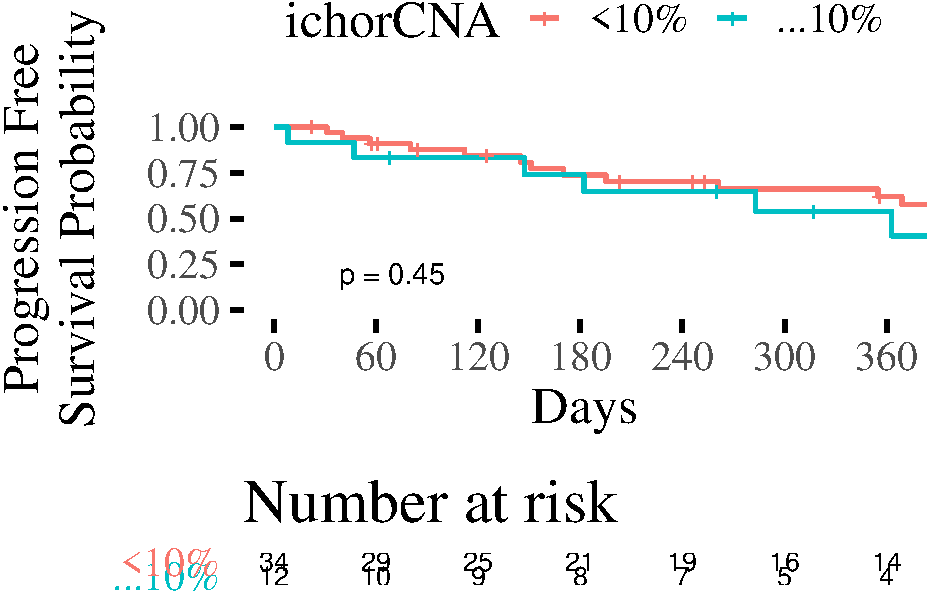
\includegraphics[width=0.5\linewidth]{detect.her2.manuscript_files/figure-latex/survival.cox.ichor.cut.plot-1} 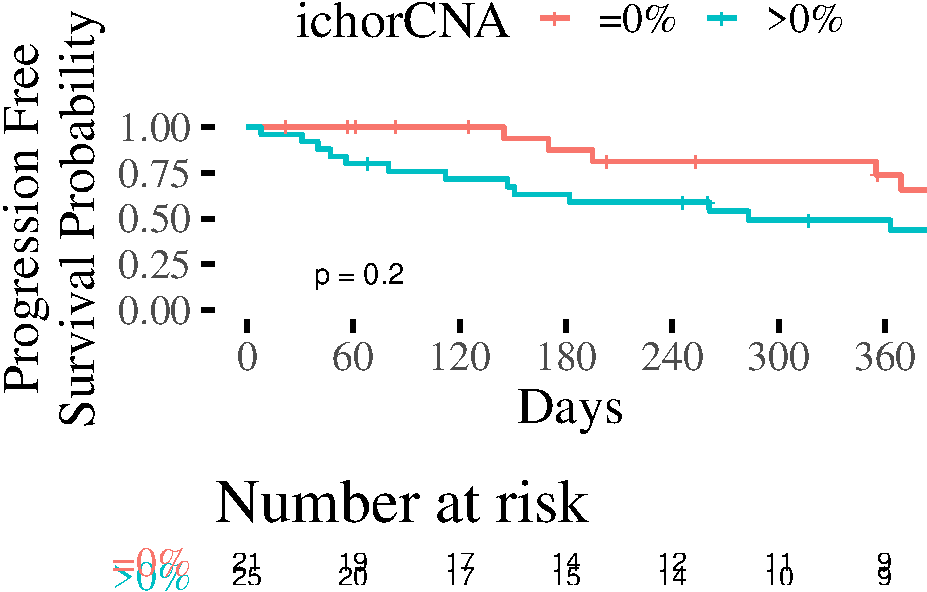
\includegraphics[width=0.5\linewidth]{detect.her2.manuscript_files/figure-latex/survival.cox.ichor.cut.plot-2} 

}

\caption{Cox propotional hazard models based on ichorCNA as a predictor}(\#fig:survival.cox.ichor.cut.plot)
\end{figure}

\begin{figure}

{\centering 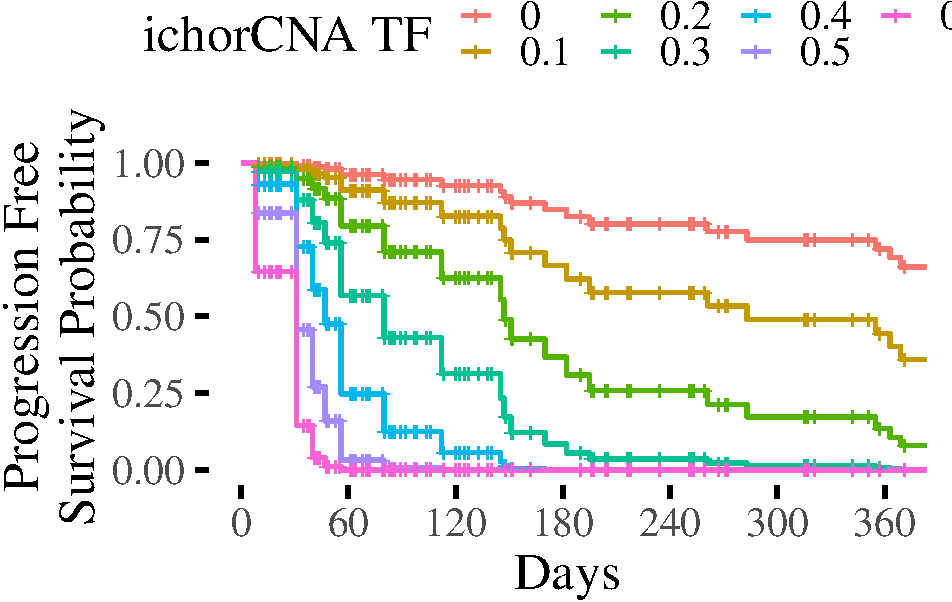
\includegraphics{detect.her2.manuscript_files/figure-latex/survival.AG.ichor.cont.plot-1} 

}

\caption{Time-dependent Cox regression using ichorCNA as a predictor}(\#fig:survival.AG.ichor.cont.plot)
\end{figure}

\begin{figure}

{\centering 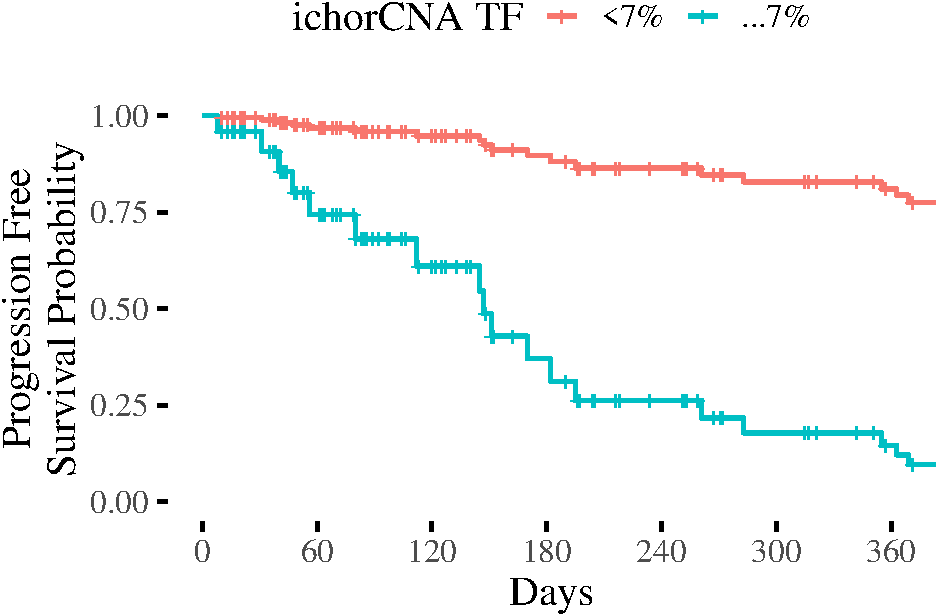
\includegraphics{detect.her2.manuscript_files/figure-latex/survival.AG.ichor.cut.plot-1} 

}

\caption{Optimal thresholding of a time-dependent Cox regression using ichorCNA as a predictor}(\#fig:survival.AG.ichor.cut.plot)
\end{figure}

\begin{figure}

{\centering 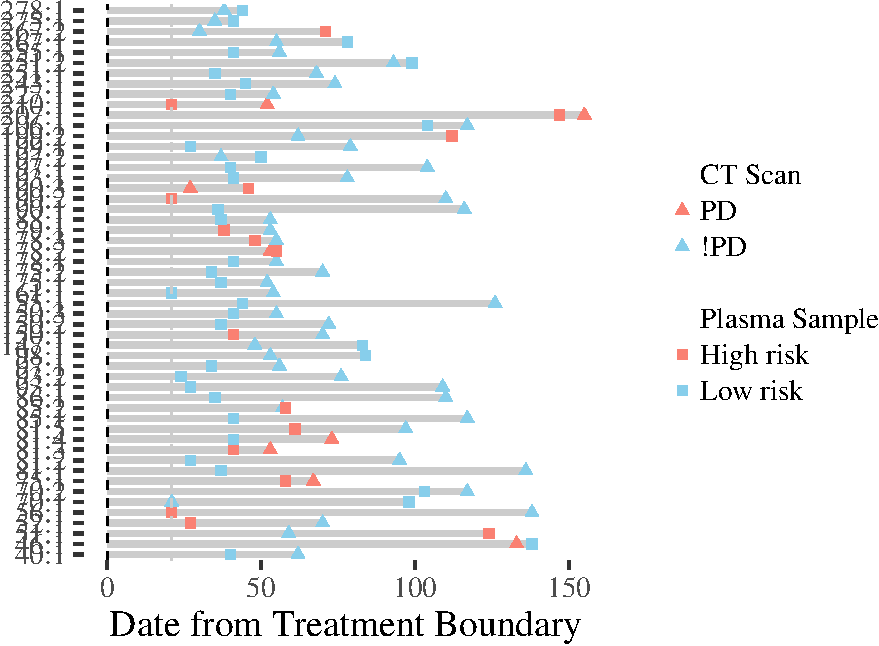
\includegraphics{detect.her2.manuscript_files/figure-latex/boundaries.overview.plot-1} 

}

\caption{Overview of treatment boundaries within DETECT Her2+ve cohort}(\#fig:boundaries.overview.plot)
\end{figure}

\begin{center}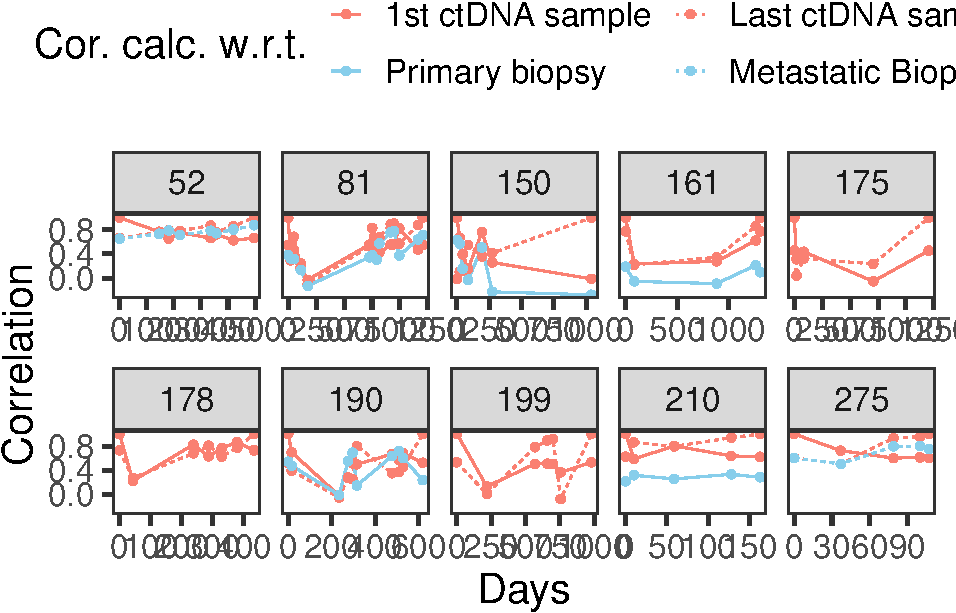
\includegraphics{detect.her2.manuscript_files/figure-latex/distance.1st_nth.plot-1} \end{center}

\begin{center}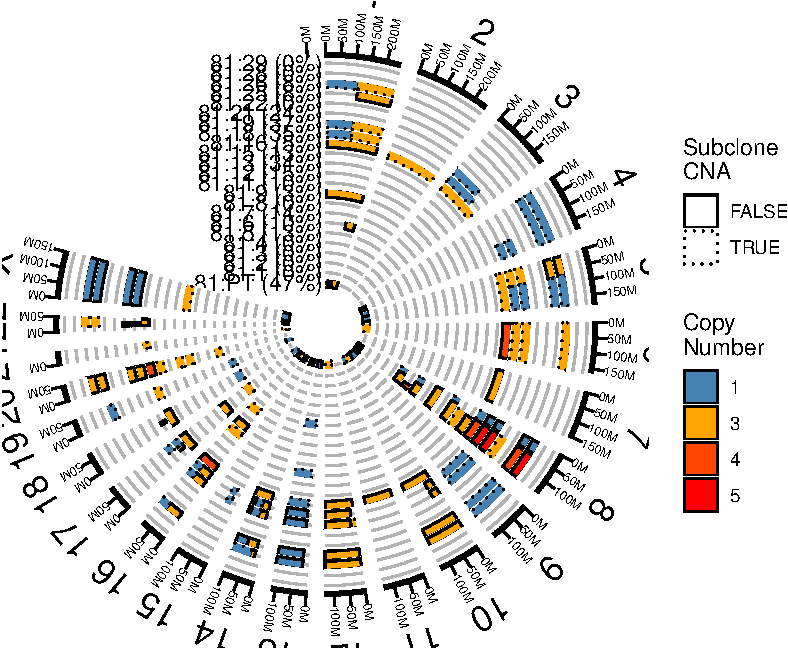
\includegraphics{detect.her2.manuscript_files/figure-latex/casestudy.circus.plot-1} \end{center}

\begin{center}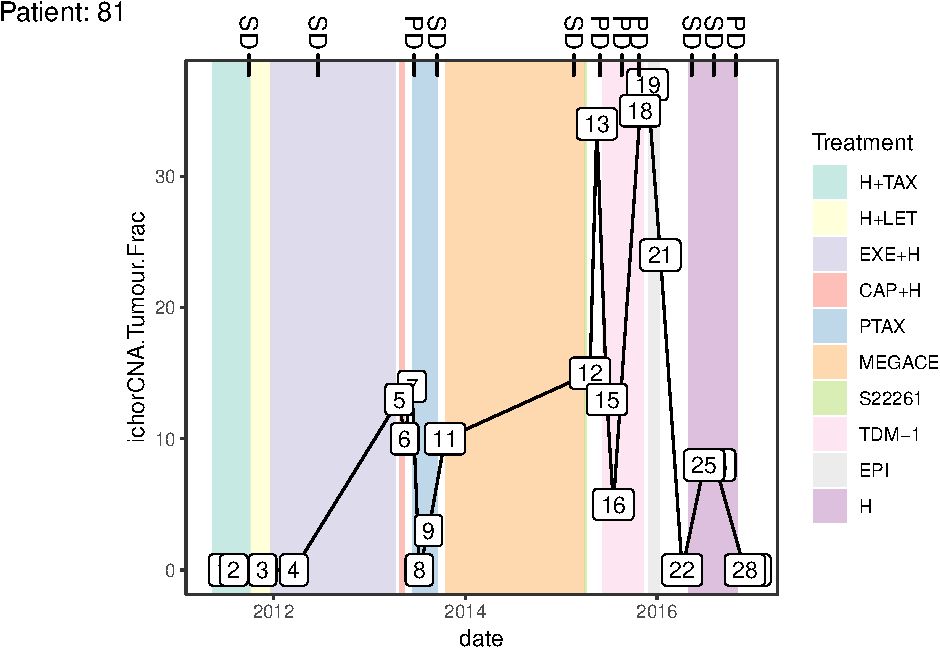
\includegraphics{detect.her2.manuscript_files/figure-latex/casestudy.timeline.plot-1} \end{center}

\begin{center}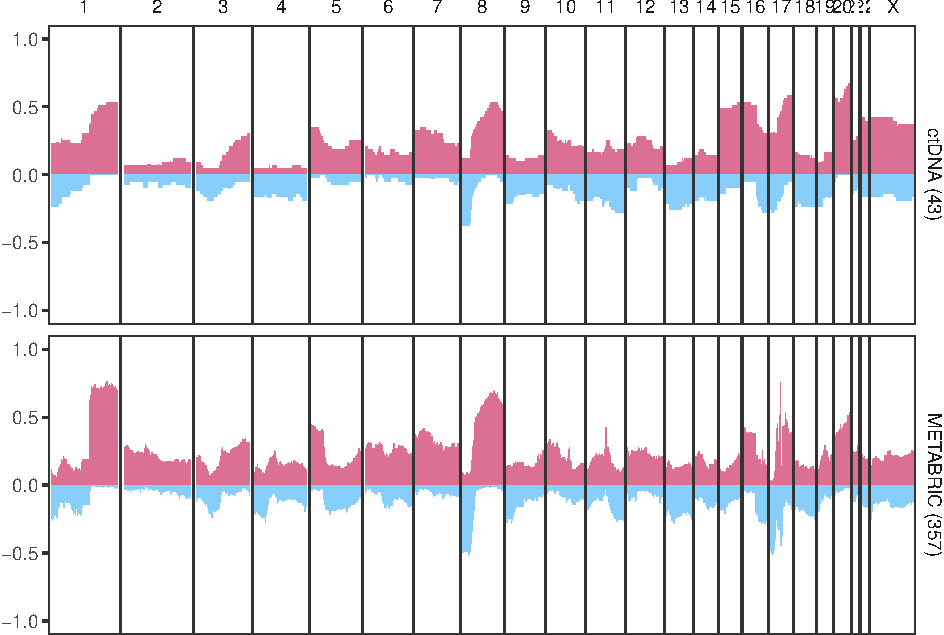
\includegraphics{detect.her2.manuscript_files/figure-latex/metabric.overview.plot-1} \end{center}

\begin{center}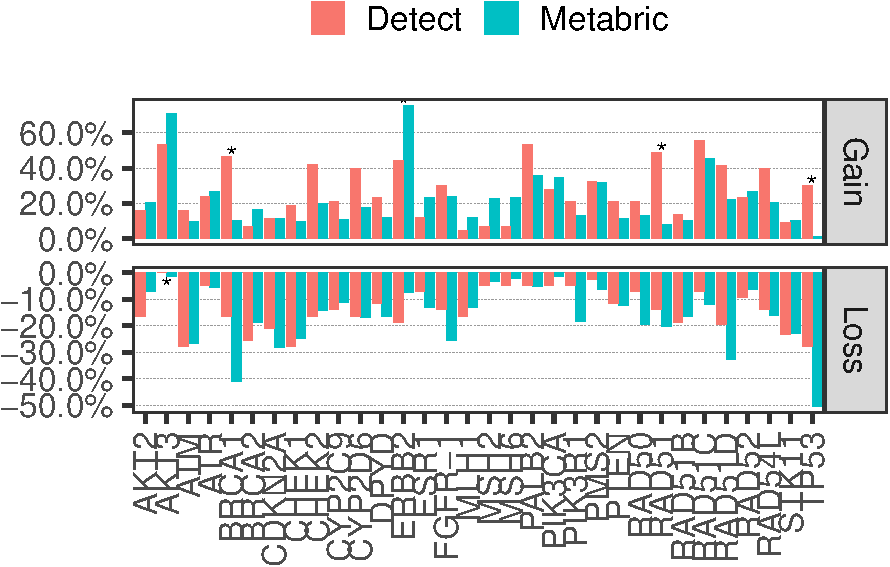
\includegraphics{detect.her2.manuscript_files/figure-latex/metabric.drivers.plot-1} \end{center}

\begin{center}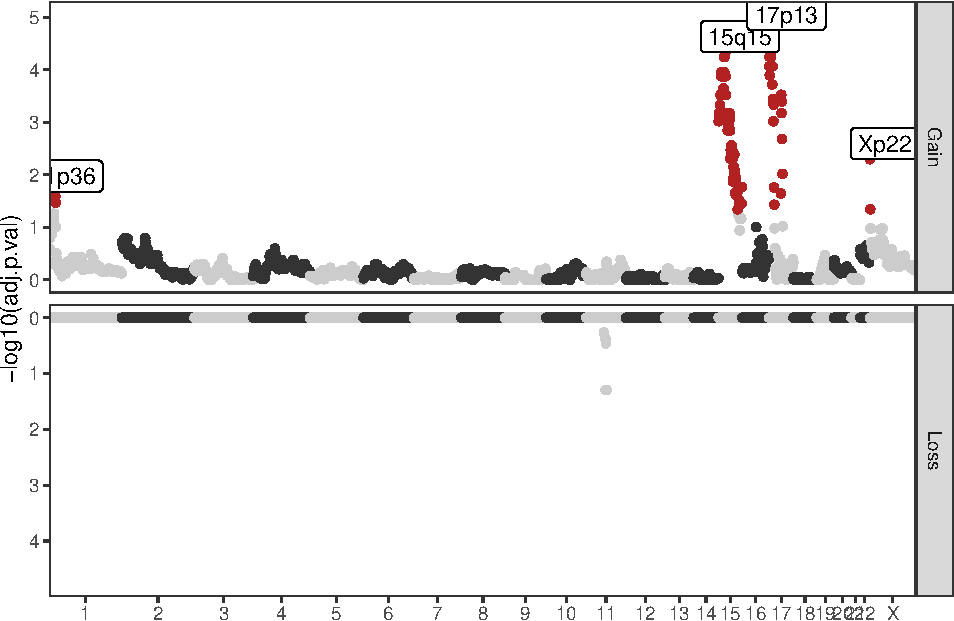
\includegraphics{detect.her2.manuscript_files/figure-latex/metabric.gwas.plot-1} \end{center}


\end{document}
